\lecture{Siemens PlantSimunlate}{18~-~01~-~2026}
%
%
\section{Panoramica}
Il software Siemens PlantSimulate permette di sincronizzare l'ingegneria di prodotto, produzione e operazioni di servizio per ottimizzare le performance produttive.

Le funzionalità principali si dividono in due macro-aree di utilizzo:
\begin{enumerate}
    \item \emph{Pianificazione di nuovi impianti}: Consente di rilevare ed eliminare problemi prima della fase di realizzazione fisica, evitando correzioni costose. Permette di determinare i limiti di performance delle macchine e dell'impianto nel suo complesso;
    \item \emph{Ottimizzazione di impianti esistenti}: Serve a migliorare le strategie di controllo, sequenziare gli ordini per minimizzare i cambi utensile e testare scenari operativi quotidiani per garantire fluidità nei processi.
\end{enumerate}
L'obiettivo finale è l'analisi statistica per ottimizzare la logistica, l'utilizzo delle macchine, il fabbisogno di manodopera e il consumo energetico, riducendo i colli di bottiglia (bottlenecks). Vedi figure \ref{fig:08-plantsim1} e \ref{fig:08-plantsim2}.
\begin{figure}
    \centering
    \begin{subfigure}{0.45\linewidth}
        \centering
        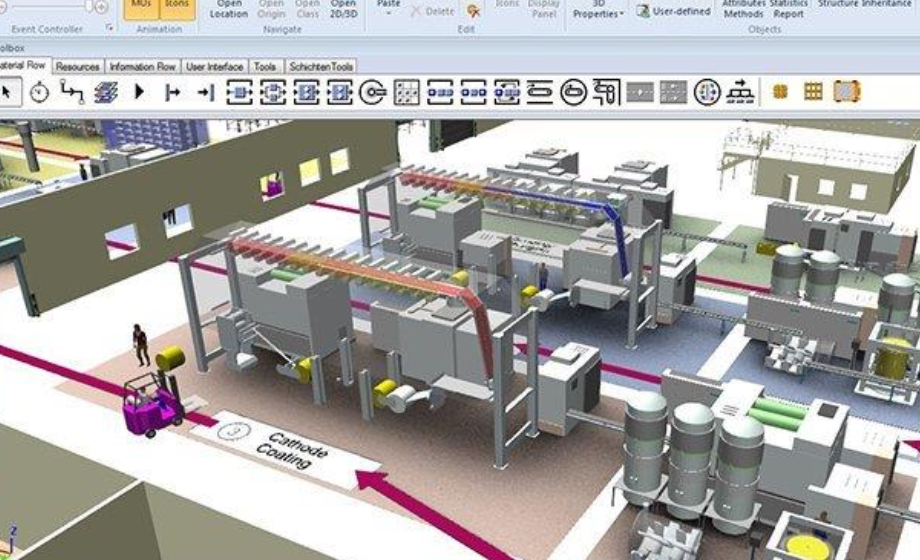
\includegraphics[width=\linewidth]{assets/Screenshot 2026-01-19 at 10.54.08.png}
        \caption{PlantSimulate}\label{fig:08-plantsim1}
    \end{subfigure}
    \begin{subfigure}{0.45\linewidth}
        \centering
        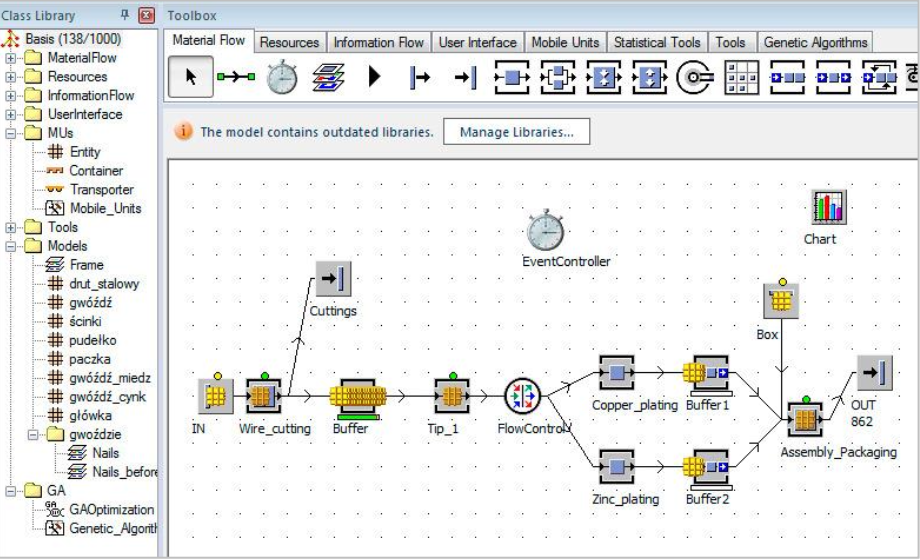
\includegraphics[width=\linewidth]{assets/Screenshot 2026-01-19 at 10.54.14.png}
        \caption{PlantSimulate}\label{fig:08-plantsim2}
    \end{subfigure}
    \caption{}\label{fig:}
\end{figure}

%
\subsection{User Interface}
L'interfaccia si basa su una Class Library che contiene oggetti predefiniti come:
\begin{itemize}
    \item Material Flow: Gestione del flusso materiali (es. nastri trasportatori);
    \item Resources: Risorse produttive;
    \item Information Flow: Flusso dati;
    \item User Interface \& Tools: Strumenti di visualizzazione e controllo.
\end{itemize}
Un elemento centrale è l'EventController, che gestisce il tempo della simulazione (Start, Stop, Reset, velocità).
%
\section{Esempi}
Adesso vediamo degli esempi di simulazione di modifiche apportabili ad una linea di produzione.
%
\subsection{Energy.Model}
Questo esempio ha l'obiettivo di ottimizzare l'utilizzo energetico di una linea di produzione semplice. Vedi figura \ref{fig:08-energy}.
\begin{figure}
    \centering
    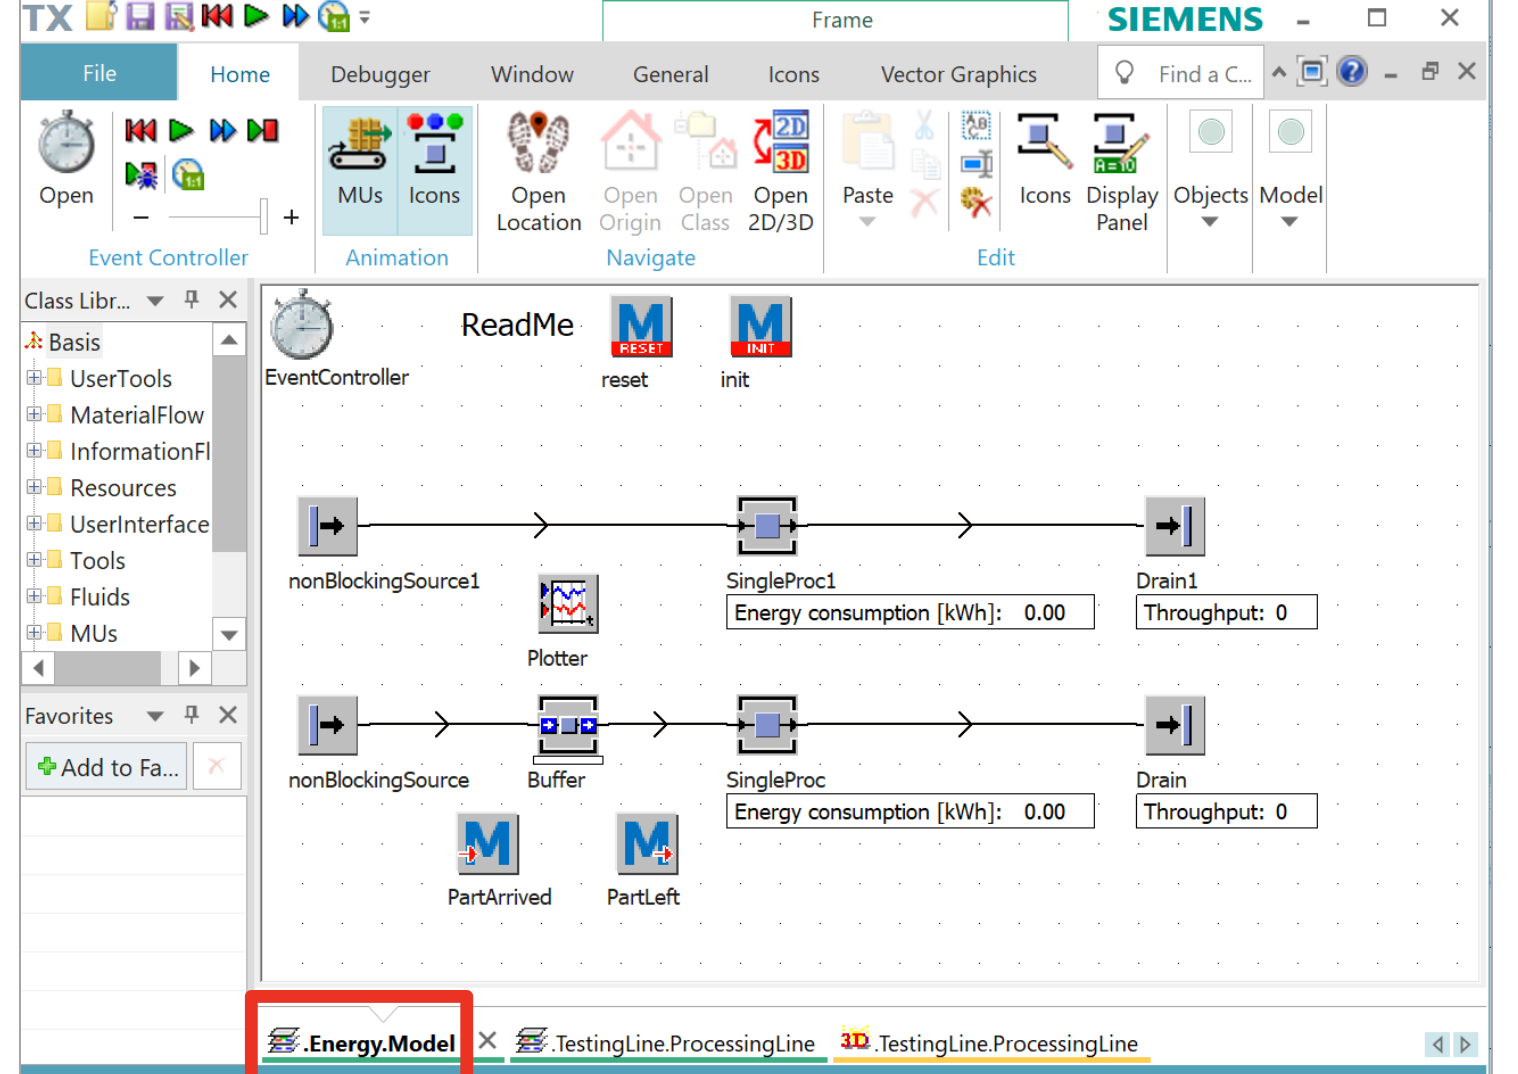
\includegraphics[width=0.8\linewidth]{assets/Screenshot 2026-01-19 at 16.41.21.png}
    \caption{Esempio di Energy Optimization applicata ad una linea di produzione.}\label{fig:08-energy}
\end{figure}
%
\paragraph{Struttura} Una sorgente (Source) invia parti a una stazione di processo (SingleProc), che poi le invia allo scarico (Drain).
%
\paragraph{Logica degli stati} La stazione SingleProc non consuma energia in modo costante, ma varia in base al suo stato operativo. Ad esempio:
\begin{itemize}
    \item \emph{Working}: 1 kW (mentre lavora il pezzo);
    \item \emph{Standby/Operational}: 0.5 kW (in attesa o attivo ma non lavorante);
    \item \emph{Off}: 0 kW.
\end{itemize}
\subsubsection{Risultato sim}
Ora si può fare il confronto dei Buffer:
\begin{itemize}
    \item \textbf{Senza Buffer}: Il consumo energetico è più alto perché la macchina, se non ha pezzi, potrebbe rimanere in stati operativi inefficienti o accendersi/spegnersi frequentemente.
    \item \textbf{Con Buffer (Capacità 12)}: Risulta più efficace. La presenza del buffer permette di accumulare pezzi; la macchina può sfruttare lo stato di Stand-by a basso consumo mentre aspetta che il buffer si riempia, ottimizzando il ciclo produttivo.
\end{itemize}
%
\subsection{TestingLine.ProcessingLine}
Questo esempio simula una linea di assemblaggio per componenti di TV e DVD. Vedi figura \ref{fig:08-prod}.
\begin{figure}
    \centering
    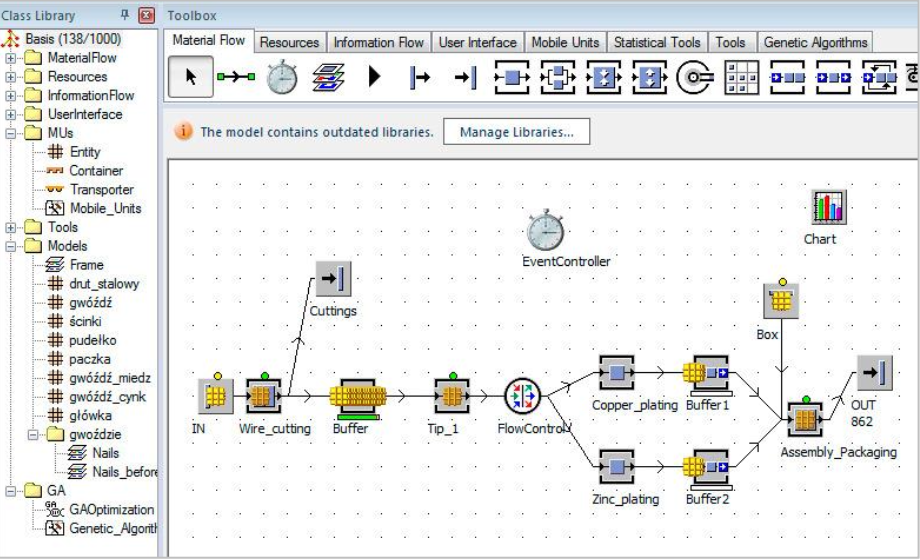
\includegraphics[width=0.8\linewidth]{assets/Screenshot 2026-01-19 at 10.54.14.png}
    \caption{TV \& DVD Production line}\label{fig:08-prod}
\end{figure}
%
\paragraph{Flusso del processo}
\begin{enumerate}
    \item Produzione mista: Una \verb|Source| produce componenti basandosi su una tabella (\verb|SourceData|) che definisce la frequenza: 70\% TV e 30\% DVD;
    \item Assemblaggio: I prodotti vengono uniti a dei contenitori (provenienti da \verb|SourceContainers|) in una stazione di caricamento (\verb|LoadingStation|);
    \item Movimentazione: I pezzi assemblati viaggiano su un convogliatore (\verb|Conveyor|).
    \item Robotica: Un braccio robotico (\verb|PickAndPlace|) preleva la parte e determina la destinazione corretta verso l'uscita.
\end{enumerate}
%
\paragraph{Output} Il modello raccoglie statistiche di produzione e offre una visualizzazione 3D del processo. Vedi figura \ref{fig:08-3d}.
\begin{figure}
    \centering
    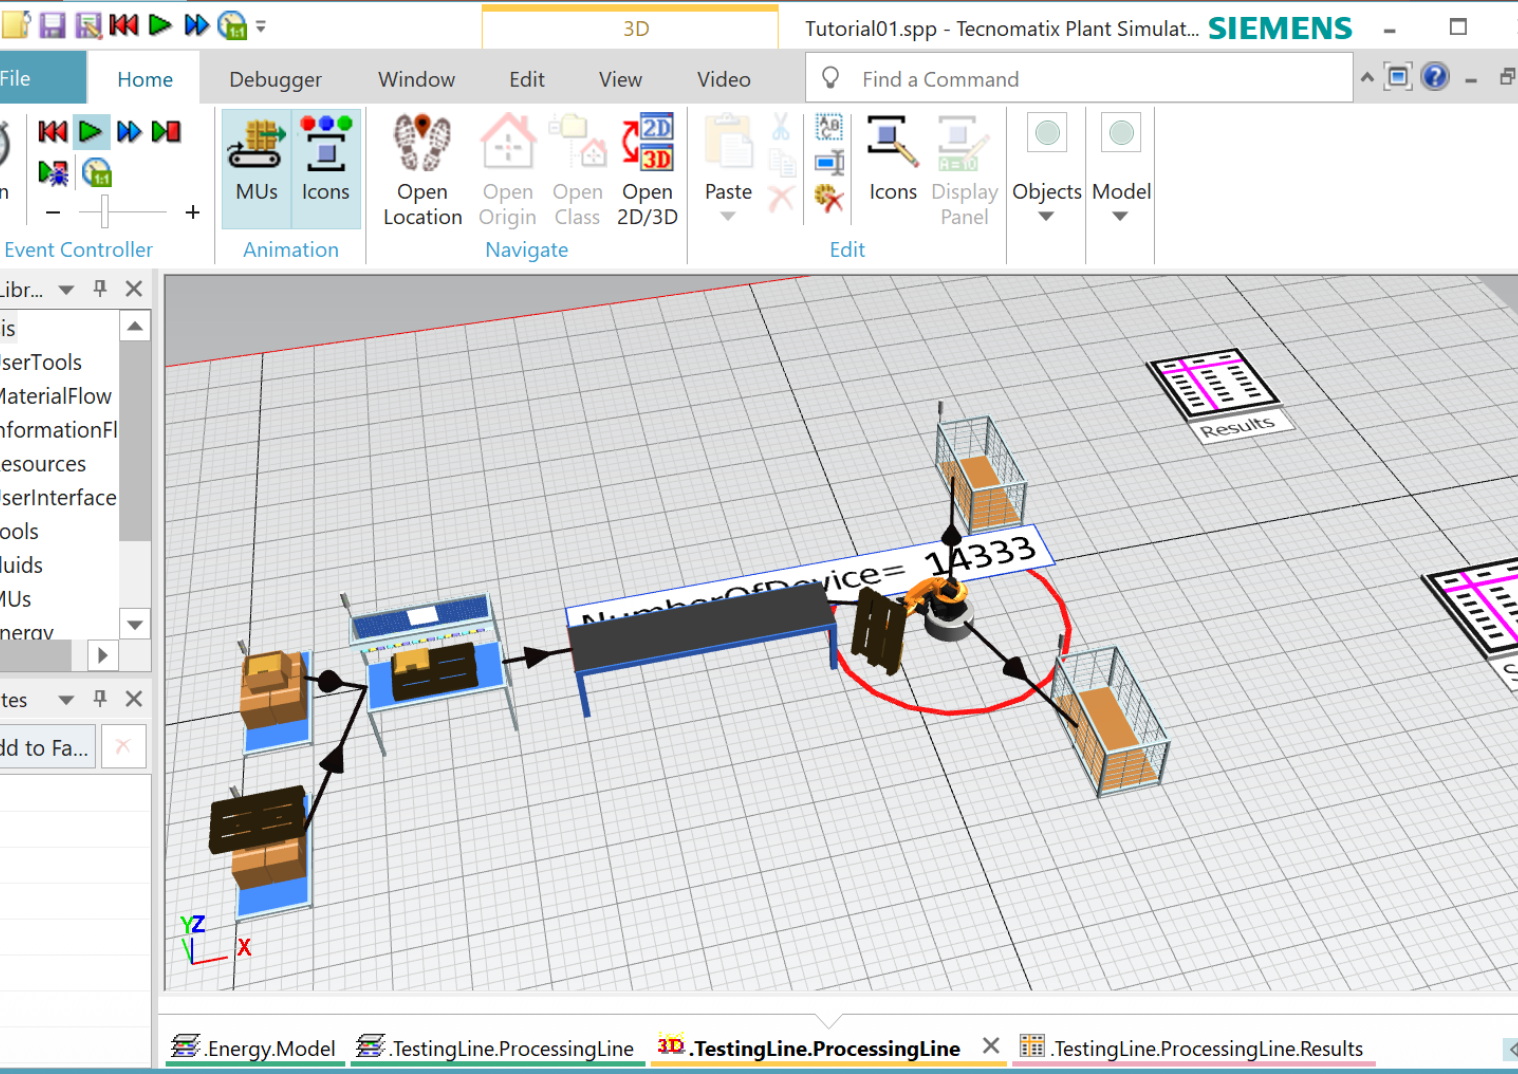
\includegraphics[width=0.8\linewidth]{assets/Screenshot 2026-01-19 at 16.46.18.png}
    \caption{3D Visualization of the output model.}\label{fig:08-3d}
\end{figure}

%
\section{Error Handling}
Durante l'apertura dei modelli, il software potrebbe presentare degli avvisi a cui è necessario rispondere affermativamente:
\begin{itemize}
    \item Richiesta di accesso al computer (poiché il modello è stato salvato da un altro utente);
    \item Avviso sulla scheda grafica (suggerimento di usare il processore NVIDIA ad alte prestazioni invece della grafica integrata CPU per performance ottimali).
\end{itemize}
Vedi le figure \ref{fig:errors}.

\begin{figure}
    \centering
    \begin{subfigure}{0.378\linewidth}
        \centering
        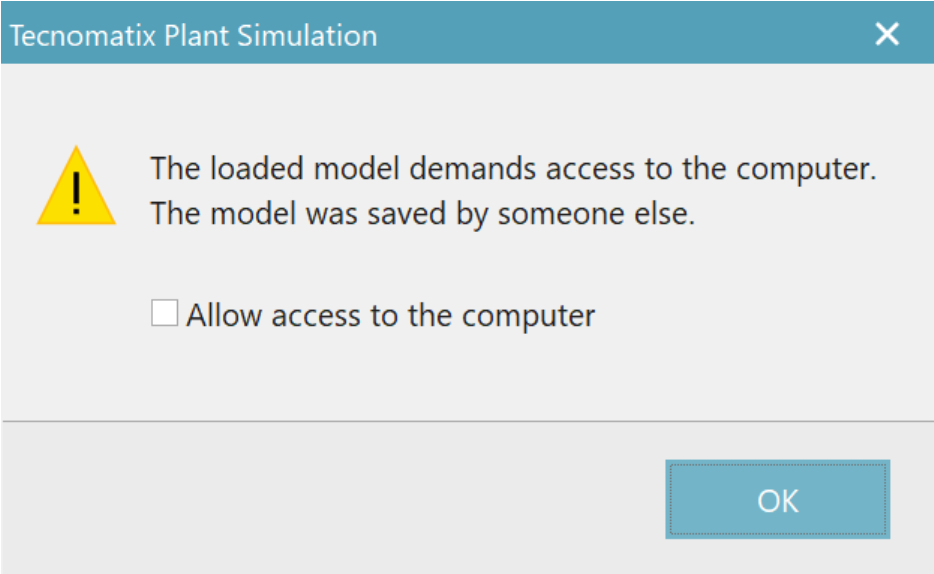
\includegraphics[width=\linewidth]{assets/Screenshot 2026-01-19 at 16.49.02.png}
        \caption{Error type 1}\label{fig:}
    \end{subfigure}
    \begin{subfigure}{0.45\linewidth}
        \centering
        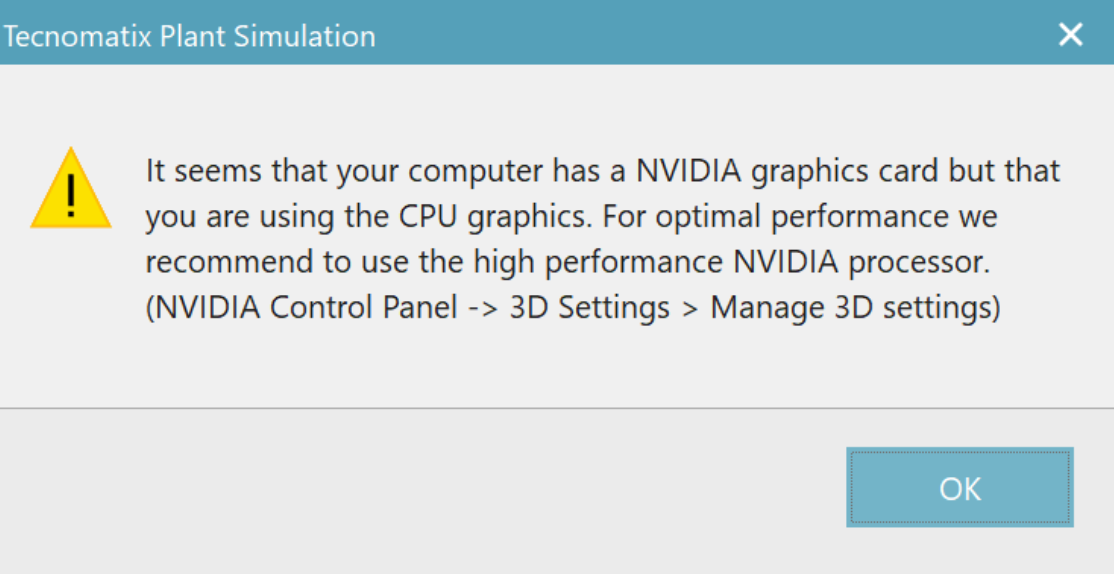
\includegraphics[width=\linewidth]{assets/Screenshot 2026-01-19 at 16.48.21.png}
        \caption{Error type 2}\label{fig:error}
    \end{subfigure}
    \caption{Select ``YES'' to both errors.}\label{fig:errors}
\end{figure}